\normaltrue \difficilefalse \tdifficilefalse
\correctionfalse

%\UPSTIidClasse{11} % 11 sup, 12 spé
%\newcommand{\UPSTIidClasse}{11}

\exer{Calcul de FTBO$\star$ \label{B2:07:505}}
\setcounter{question}{0}\marginnote{\xpComp{SLCI}{03}}%\UPSTIcompetence{B2-07}
\index{Compétence B2-07}\index{Compétence SLCI-03}
\index{Schéma-blocs}
\index{FTBO}

\ifcorrection
\else
\marginnote{\textbf{Pas de corrigé pour cet exercice.}}
\fi


\question{Déterminer la FTBO dans la cas suivant.}
\ifprof 
$\text{FTBO}(p) = BCDE$.
\else
\begin{marginfigure}
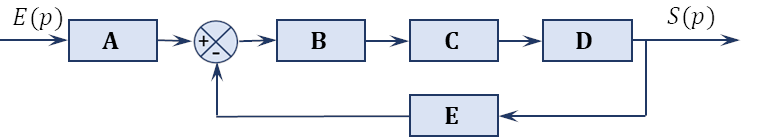
\includegraphics[width=\linewidth]{505_01}
\end{marginfigure}
\fi
 
\question{Déterminer la FTBO dans la cas suivant.}
\ifprof 
$\text{FTBO}(p) = B\left(1+A\right)$.
\else
\begin{marginfigure}
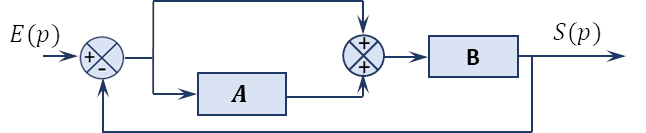
\includegraphics[width=\linewidth]{505_02}
\end{marginfigure}
\fi

\question{Déterminer la FTBO dans la cas suivant.}
\ifprof 
$\text{FTBO}(p) = A \dfrac{BCD}{1+BCD}$.
\else
\begin{marginfigure}
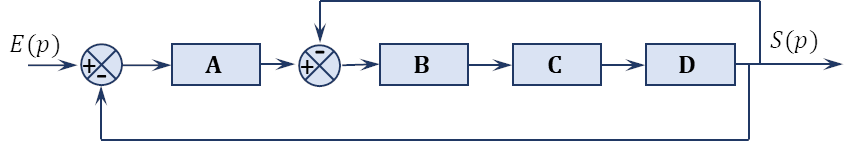
\includegraphics[width=\linewidth]{505_03}
\end{marginfigure}
\fi

\question{Déterminer la FTBO dans la cas suivant.}
\ifprof 
$\text{FTBO}(p) = A \dfrac{\dfrac{B}{1+B}CD}{1+\dfrac{B}{1+B}CD} = \dfrac{ABCD}{1+B+BCD}$.
\else
\begin{marginfigure}
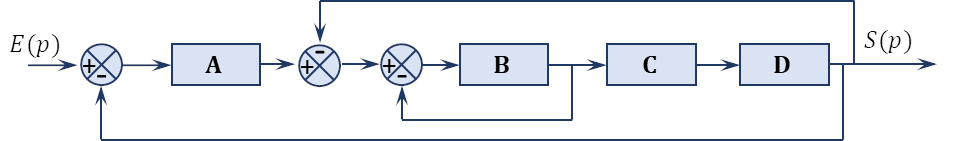
\includegraphics[width=\linewidth]{505_04}
\end{marginfigure}
\fi



%\question{Réaliser le schéma-blocs.}
%\ifprof
%\begin{marginfigure}
%\centering
%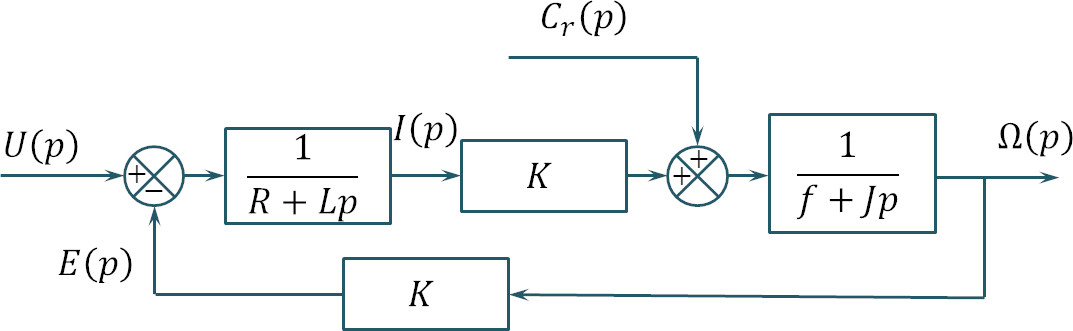
\includegraphics[width=\linewidth]{51_01_c}
%%\caption{Évolution du couple utile en fonction de la vitesse de rotation pour des
%%fréquences de commande de \SI{90}{Hz} à \SI{110}{Hz}. \label{fig_50_04}}
%\end{marginfigure}
%\else
%\fi


 

\ifprof
\else
\begin{solution}
\begin{enumerate}
\item $\text{FTBO}(p) = BCDE$.
\item $\text{FTBO}(p) = B\left(1+A\right)$.
\item $\text{FTBO}(p) = A \dfrac{BCD}{1+BCD}$.
\item $\text{FTBO}(p) = \dfrac{ABCD}{1+B+BCD}$.
\end{enumerate}
\end{solution}

\marginnote{Corrigé voir \ref{B2:07:505}.}

\fi